% ===========================================================================
% DeepONet-Based Neural Network for Thomson Scattering Profile Fitting on EAST
% Target: Plasma Science and Technology (PST) / Fusion Engineering and Design
% ===========================================================================

\documentclass[a4paper,12pt]{article}

% ---- Packages ----
\usepackage{amsmath,amssymb}
\usepackage{graphicx}
\usepackage{booktabs}
\usepackage{multirow}
\usepackage{hyperref}
\usepackage[margin=2.5cm]{geometry}
\usepackage{caption}
\usepackage{subcaption}
\usepackage{microtype}
\microtypesetup{expansion=false}  % disable font expansion for compatibility
\usepackage{enumitem}

% Relaxed spacing for narrow columns
\sloppy
\hyphenpenalty=1000
\tolerance=2000

% ---- Metadata ----
\title{DeepONet-Based Neural Network for Thomson Scattering \\ Profile Fitting on EAST Tokamak}

\author{%
C.Y. Hu$^{1,2,3}$, Q. Zang$^{3,\ast}$\thanks{Project supported by [funding information to be added]. Corresponding author: Q. Zang (zangq@ipp.ac.cn).} \\[4pt]
$^1$ Anhui University of Science and Technology, Huainan 232001, China \\
$^2$ Institute of Energy, Hefei Comprehensive National Science Center \\
(Anhui Energy Laboratory), Hefei 230031, China \\
$^3$ Institute of Plasma Physics, Chinese Academy of Sciences, \\
Hefei 230031, China
}

\date{\today}

\begin{document}
\maketitle

\begin{abstract}
\small
Thomson Scattering (TS) diagnostics on the EAST tokamak provide discrete measurements of electron temperature (Te) and density (ne) at 20--30 spatial channels. Reconstructing continuous radial profiles from these scattered points is a prerequisite for transport analysis and equilibrium reconstruction. The widely used modified hyperbolic tangent (mtanh) method relies on diagnostic-specific processing branches and hand-tuned parameters, limiting scalability to the thousands of discharges produced annually. We propose a DeepONet-based neural network approach that replaces the seven-step mtanh pipeline with a single 14 ms forward pass. Models are trained on (scattered points, mtanh-fitted profile) pairs from 161 EAST discharges (2015--2024 campaigns). We compare five architectures. ProfileNet (SetEncoder), BiLSTM, Transformer, and CNN-DeepONet share one CoordDecoder (trunk net) and one physics-constrained loss; a pure CNN-1D without the branch-trunk structure serves as a control. On a test set of 4 unseen EAST shots (20 time points, 300 profiles) spanning L-mode to strong H-mode conditions (Te = 0.2--7.2 keV), the neural networks achieve mean absolute errors of Te = 0.36--0.53 keV, ne = 0.05--0.11 (in units of 10\textsuperscript{19} m\textsuperscript{-3}), and ion temperature Ti = 0.07--0.14 keV relative to the mtanh baseline.

Ablation experiments point to a key architectural distinction: with the physics constraints removed, the pure CNN-1D degrades by 30.9\%, but the DeepONet models improve slightly ($-$11.5\%). The reason is the branch--trunk dot product itself: every output is a linear combination of smooth basis functions, so smoothness comes from the architecture instead of penalty terms. A controlled CNN-DeepONet variant (the CNN encoder paired with the shared trunk) resolves the encoder/decoder confound: the trunk decoder improves Ti substantially (0.142 to 0.082 keV) but does nothing for Te or ne, so the regularization is diagnostic-specific. No single architecture is optimal for all diagnostics; the differences track how each diagnostic samples space, not model capacity. Where earlier studies tested one ML model at a time, this work compares five architectures under identical training and evaluation conditions. We therefore recommend a diagnostic-matched ensemble (CNN-Te + Transformer-ne + LSTM-Ti, total inference $<$50 ms).

\textbf{Keywords}: EAST tokamak, Thomson scattering, profile fitting, DeepONet, neural network, physics-constrained learning

\noindent\textbf{PACS:} 52.55.Fa, 52.70.Kz, 07.05.Mh
\end{abstract}

% ===========================================================================
% 1. Introduction
% ===========================================================================
\section{Introduction}

The Experimental Advanced Superconducting Tokamak (EAST) at the Institute of Plasma Physics, Chinese Academy of Sciences (ASIPP), is a fully superconducting tokamak dedicated to long-pulse, high-performance plasma operation~\cite{east_overview}. Understanding the spatial structure of kinetic profiles---electron temperature $T_e(\rho)$, electron density $n_e(\rho)$, and ion temperature $T_i(\rho)$ as functions of the normalized minor radius $\rho$---is essential for transport analysis and equilibrium reconstruction. EAST's Thomson Scattering (TS) diagnostic measures $T_e$ and $n_e$ at $\sim$20--30 spatial channels~\cite{east_ts,east_tvts}, supplemented by a Reflectometer (Refl) for higher-resolution $n_e$ and an X-ray Crystal Spectrometer (TXCS) for $T_i$. These discrete scattered points must be reconstructed into continuous profiles before they can be used in codes such as ONETWO~\cite{onetwo} or TRANSP.

The standard profile fitting method on EAST employs a modified hyperbolic tangent (mtanh) function~\cite{mtanh_groebner}, which partitions the profile into a core spline region ($\rho < 0.85$) and a pedestal mtanh region ($\rho > 0.85$) connected by a smooth transition. The method is physically motivated and widely validated, but in practice it has real limitations. The pipeline is a seven-step chain (IQR outlier removal, core spline fitting, pedestal mtanh optimization, smooth transition, left-boundary correction) realized as six diagnostic-specific code branches. Every branch carries hand-tuned parameters (pedestal position, IQR thresholds, spline knots) that can fail on unusual discharges; every fit must be checked by eye; and the pedestal least-squares optimization is sensitive to its starting point. These issues limit scalability to EAST's annual output of thousands of discharges.

Machine learning has reached fusion diagnostics as well: Gaussian Process Regression for profile fitting~\cite{gpr_profiles,gpr_review}, Bayesian integrated data analysis~\cite{ida_east}, neural networks for TS temporal super-resolution~\cite{diag2diag}, and CNN-based density profile reconstruction~\cite{lan_cnn_east}. The Deep Operator Network (DeepONet)~\cite{deeponet} is a neural architecture specifically designed to learn mappings between function spaces, separating an operator $G: u \mapsto G(u)$ into a branch network encoding the input function and a trunk network encoding the output domain~\cite{physics_informed_deeponet,pinn_review}. The branch-trunk form has one property we rely on throughout: the output $\hat{y}(\rho) = \sum b_k \cdot t_k(\rho)$ is always a linear combination of smooth basis functions. Non-physical oscillations are excluded by construction, and we treat the architecture itself as \textit{structural regularization} for profile fitting.

In this work, we propose a DeepONet-based neural network that replaces the seven-step mtanh pipeline with a single $\sim$14 ms forward pass. Five architectures are compared---four (ProfileNet (SetEncoder), BiLSTM, Transformer, and CNN-DeepONet) share a common CoordDecoder and physics-constrained loss, while a pure CNN-1D serves as a control group without the branch-trunk structure---enabling a controlled study of architectural inductive biases. Our contributions include: (1) first application of DeepONet to EAST TS profile fitting; (2) systematic five-architecture comparison under unified conditions; (3) a controlled CNN-DeepONet variant that resolves the encoder/decoder confound, showing the shared trunk decoder is beneficial for sparse diagnostics (Ti) but not dense ones (Te, ne); (4) ablation experiments showing the branch-trunk structure regularizes by itself (without physics constraints CNN-1D degrades 30.9\%, whereas the DeepONet architectures improve slightly); (5) discovery of a diagnostic-architecture matching pattern reflecting intrinsic differences in diagnostic spatial sampling; and (6) quantification of downstream LHW current drive impact ($\sim$24\% deviation from mtanh).

% ===========================================================================
% 2. Method
% ===========================================================================
\section{Method}

\subsection{Problem Formulation}

Given $N$ discrete diagnostic measurements $\{(\rho_i, y_i)\}_{i=1}^N$, where $\rho_i \in [0, 1]$ is the normalized minor radius and $y_i$ is the physical quantity ($T_e$ in eV, $n_e$ in $10^{19}$ m$^{-3}$, or $T_i$ in keV), with $N$ typically ranging from 5 to 35 depending on the diagnostic, the goal is to learn a mapping $\mathcal{F}$ that outputs a smooth profile $\hat{y}(\rho)$ evaluated on a uniform grid of 201 points over $\rho \in [0, 1]$.

The mtanh approach implements $\mathcal{F}$ through an explicit parametric pipeline: IQR outlier removal $\to$ core spline fitting $\to$ pedestal mtanh parameter optimization $\to$ smooth transition $\to$ left-boundary correction. In contrast, the neural network approach learns $\mathcal{F}$ implicitly through supervised learning on a dataset of (scattered points, fitted profile) pairs.

\subsection{Training Data}

Training data were constructed from EAST discharges spanning 2015--2024 campaigns (161 shots, shot numbers 60150--149600). For each (shot, time) pair with available diagnostic data, the standard mtanh pipeline was executed to produce a 201-point fitted profile serving as the training label. The raw scattered diagnostic points---without IQR cleaning---serve as the neural network input. Invalid channels (non-finite readings or values below diagnostic-specific validity thresholds) are masked out when the scatter input is constructed; all encoders natively accept variable-length point sets, and CNN-1D additionally encodes the mask as a second input channel.

\textbf{H-mode/L-mode classification}: The energy confinement factor $H_{98}$ was read from the EAST MDSplus \texttt{energy\_east} tree ($\backslash$H98\_MHD signal). Time points with $H_{98} \geq 0.7$ are classified as H-mode, $0 < H_{98} < 0.7$ as L-mode, and $H_{98} = 0$ as unknown (data unavailable).

\textbf{Stratified shot-based split}: To prevent data leakage, all time points from the same discharge are assigned to the same dataset partition (train/validation/test). The split ratio is 70/15/15, stratified by plasma mode where possible. The test set consists of 4 unseen 2024 shots (156005, 156010, 156100, 156400) covering L-mode to strong H-mode conditions ($T_e = 0.2$--$7.2$ keV). Key test set statistics are summarized in Table~\ref{tab:testset}.

\begin{table}[htbp]
\centering\footnotesize
\caption{Test set characteristics. All 4 shots are from the 2024 EAST campaign and are excluded from the training set.}
\label{tab:testset}
\resizebox{\textwidth}{!}{%
\begin{tabular}{ccccccc}
\toprule
\textbf{Shot} & \textbf{Time Points} & \textbf{$T_e$ Range (keV)} & \textbf{Mode (H/L/unk)} & \textbf{$H_{98}$ Range} & \textbf{TS} & \textbf{Refl+TXCS} \\
\midrule
156005 & 2 & 0.6--2.4 & 1H / 1L & 0.69--0.96 & \checkmark & \checkmark \\
156010 & 6 & 0.2--2.3 & 6 unknown & 0.0$^*$ & \checkmark & \checkmark \\
156100 & 6 & 1.2--3.3 & 1H / 5L & 0.56--1.10 & \checkmark & \checkmark \\
156400 & 6 & 3.8--7.2 & 6H & 0.85--1.15 & \checkmark & \checkmark \\
\midrule
Total & 20 & 0.2--7.2 & 8H / 6L / 6unk & --- & 20 & 20 \\
\bottomrule
\end{tabular}%
}
\vspace{4pt}
\footnotesize{$^*$ Shot 156010: $H_{98}$ data unavailable from MDSplus (returns 0.0). Plasma mode is marked as ``unknown.''}
\end{table}

\subsection{Model Architecture}

Four of the five architectures share a common DeepONet-style decoder and differ only in the encoder design (Figure~\ref{fig:architecture}); the fifth, CNN-1D, uses a pure convolutional decoder as a control. The shared \textbf{CoordDecoder} (trunk net) is an MLP(1$\to$128$\to$128, SiLU) that maps the output coordinate $\rho$ to a set of basis functions $\mathbf{b}(\rho) \in \mathbb{R}^{128}$. The final output is:
\begin{equation}
\hat{y}(\rho) = \text{Softplus}\left(\mathbf{z} \cdot \mathbf{b}(\rho)\right) = \text{Softplus}\left(\sum_{k=1}^{128} z_k \cdot b_k(\rho)\right)
\label{eq:dotproduct}
\end{equation}
where $\mathbf{z} \in \mathbb{R}^{128}$ is the latent vector produced by the encoder. The Softplus activation ($\ln(1 + e^x)$) ensures positivity of the predicted physical quantities.

\begin{figure}[htbp]
\centering
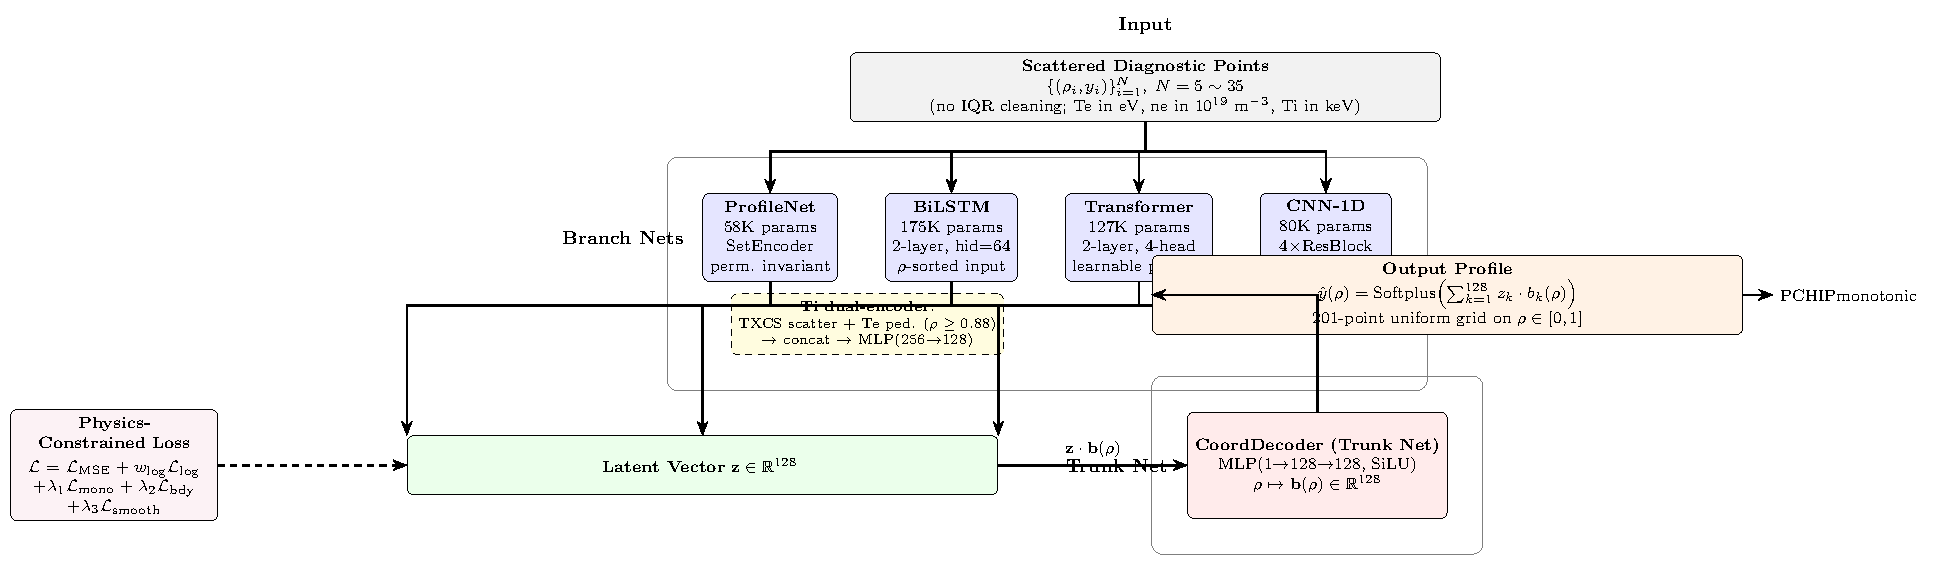
\includegraphics[width=\textwidth]{fig1_architecture.pdf}
\caption{DeepONet-based architecture for TS profile fitting. Four DeepONet encoder variants (branch nets)---ProfileNet, BiLSTM, Transformer, and CNN-DeepONet---encode scattered diagnostic points into a latent vector $\mathbf{z}$. A shared CoordDecoder (trunk net) maps the output coordinate $\rho$ to smooth basis functions $\mathbf{b}(\rho)$. The dot product $\mathbf{z}\cdot\mathbf{b}(\rho)$, followed by Softplus activation, produces the continuous profile $\hat{y}(\rho)$. A fifth architecture, CNN-1D, uses pure convolutional encoder--decoder layers without the branch-trunk structure, serving as a control group. Ti models use a dual-encoder design (TXCS scatter + Te pedestal). Training is supervised by a physics-constrained loss combining region-weighted MSE with monotonicity, boundary, and smoothness penalties.}
\label{fig:architecture}
\end{figure}

\begin{figure}[htbp]
\centering
\includegraphics[width=0.95\textwidth]{paper_results/figures/fig2_hmode_overlay.png}
\caption{Typical H-mode profile fitting results: six methods (mtanh baseline + five NN architectures) compared on three representative H-mode time points across Te, ne, and Ti diagnostics.}
\label{fig:hmode}
\end{figure}

\subsubsection{Encoder Architectures}

\textbf{ProfileNet (67K parameters)}: A PointNet-style SetEncoder~\cite{pointnet} with permutation-invariant max-pooling that processes each scattered point independently through an MLP, aggregates via max-pooling, and projects to $\mathbf{z}$. The architecture is permutation-invariant---the order of diagnostic points does not affect the output.

\textbf{LSTM (76K parameters)}: A single-layer bidirectional LSTM~\cite{lstm} (hidden=64) processes the scattered points sorted by $\rho$. The final forward and backward hidden states are concatenated and projected to $\mathbf{z}$. The BiLSTM captures sequential radial structure along the $\rho$-coordinate.

\textbf{Transformer (136K parameters)}: A 2-layer TransformerEncoder~\cite{transformer} (4-head self-attention, hidden=64) with learnable positional encodings processes sorted points. Self-attention allows each diagnostic channel to directly attend to any other channel, capturing global correlations.

\textbf{CNN-DeepONet (79K parameters)}: A CNN encoder---Conv1d stem, 3$\times$ ResidualBlock1D, and a global max-pool---that matches CNN-1D's encoder, but terminates in the shared CoordDecoder via the branch-trunk dot product. This variant was introduced to resolve a confound in the original comparison: CNN-1D differed from the other three models in \textit{both} encoder and decoder, so its inferior performance could not be attributed to either component alone. Pairing a CNN encoder with the shared trunk isolates the decoder's contribution.

\textbf{CNN-1D (66K parameters, control group)}: A pure 1D ResNet with 4$\times$ ResidualBlock1D. \textbf{This architecture intentionally does not use the DeepONet branch-trunk structure.} Instead, scattered points are linearly interpolated to a 201-point grid, stacked as a 2-channel tensor [values, mask], and processed through Conv1d encoder-decoder layers with residual connections. No BatchNorm is used. Together with CNN-DeepONet, this pair isolates the effect of the branch-trunk decoder under an otherwise identical CNN encoder.

\subsubsection{Ti Dual-Encoder}

All architectures use a dual-encoder design for $T_i$: one encoder processes the TXCS scattered points (main), while a second encoder processes $T_e$ pedestal data ($\rho \geq 0.88$). The two latent vectors are concatenated and fused via MLP(256$\to$128$\to$128). This design mirrors the mtanh practice of using $T_e$ pedestal information to constrain $T_i$ edge fitting.

\subsection{Physics-Constrained Loss Function}

The training objective combines a region-weighted MSE with physics-inspired auxiliary terms:

\begin{equation}
\mathcal{L} = \mathcal{L}_{\text{MSE}} + w_{\log} \mathcal{L}_{\log} + \lambda_1 \mathcal{L}_{\text{mono}} + \lambda_2 \mathcal{L}_{\text{bdy}} + \lambda_3 \mathcal{L}_{\text{smooth}}
\label{eq:loss}
\end{equation}

\begin{itemize}
    \item $\mathcal{L}_{\text{MSE}}$: Region-weighted MSE (core $\rho < 0.85$: 3$\times$, pedestal $\rho \geq 0.85$: 25$\times$), prioritizing accurate pedestal reconstruction.
    \item $\mathcal{L}_{\log}$ ($w_{\log}=0.1$): Log-space MSE, penalizing relative errors in low-value edge regions where absolute errors are naturally small but physically significant.
    \item $\mathcal{L}_{\text{mono}}$ ($\lambda_1=0.05$): $\text{ReLU}(d\hat{y}/d\rho)$, penalizing only positive derivatives (non-monotonic segments). Does not enforce global monotonicity; only suppresses local non-physical increases.
    \item $\mathcal{L}_{\text{bdy}}$ ($\lambda_2=0.05$): Minimizes $|d\hat{y}/d\rho|$ for $\rho < 0.05$, enforcing the magnetic axis symmetry condition $dT/d\rho|_{\rho=0} = 0$.
    \item $\mathcal{L}_{\text{smooth}}$ ($\lambda_3=0.01$): Penalizes large second derivatives $|d^2\hat{y}/d\rho^2|$, suppressing high-frequency oscillations.
\end{itemize}

The penalty weights ($\lambda_1$, $\lambda_2$, $\lambda_3$, $w_{\log}$) were set empirically on the validation set and are kept identical across all architectures to preserve comparability; their influence is examined directly in the ablation study (Table~\ref{tab:ablation}).

\subsection{Training Details}

All models are trained with AdamW optimizer (learning rate $10^{-3}$, weight decay $10^{-5}$), cosine annealing learning rate schedule, batch size 64, and a maximum of 500 epochs with early stopping (patience = 100). Post-inference, a PCHIP (Piecewise Cubic Hermite Interpolating Polynomial) shape-preserving interpolation is applied to enforce strict monotonic decrease and floor-value edge protection. All reported metrics are evaluated on the profiles after this post-processing step. Inference times are measured on CPU (10 warm-up runs followed by 200 timed passes through the full inference function, model loading excluded).

% ===========================================================================
% 3. Results
% ===========================================================================
\section{Results}

\subsection{Fitting Accuracy: Five Architectures vs. mtanh}

Table~\ref{tab:metrics} presents the overall fitting accuracy of the five neural network architectures relative to the mtanh baseline across all 20 test time points (300 total profiles). The mean absolute error (MAE) is the primary metric. Because absolute errors are not directly comparable across plasma modes (the H-mode test shots reach $T_e$ up to 7.2 keV), mean relative errors (MeanRel\%) are reported by mode in the Appendix (Table~\ref{tab:meanrel}); RMSE and MaxAE, which exhibit the same architecture rankings as MAE, are available in the supplementary material (\texttt{paper\_results/all\_metrics.csv}).

\begin{table}[htbp]
\centering\footnotesize
\caption{Fitting accuracy (MAE $\pm$ std) of NN methods relative to mtanh baseline, by diagnostic and plasma mode. Best value in each row is \textbf{bold}. H-mode: 8 time points; L-mode: 6 time points; All: 20 time points (including 6 unknown-mode).}
\label{tab:metrics}
\resizebox{\textwidth}{!}{%
\begin{tabular}{c c | c c c c c}
\toprule
\textbf{Diag.} & \textbf{Mode} & \textbf{ProfileNet} & \textbf{LSTM} & \textbf{CNN-1D} & \textbf{CNN-DeepONet} & \textbf{Transformer} \\
\midrule
\multirow{3}{*}{Te (keV)}
    & All   & 0.531$\pm$0.280 & \textbf{0.358$\pm$0.196} & 0.375$\pm$0.302 & 0.436$\pm$0.334 & 0.374$\pm$0.332 \\
    & H     & 0.639$\pm$0.230 & 0.525$\pm$0.151 & 0.661$\pm$0.278 & 0.755$\pm$0.287 & 0.694$\pm$0.299 \\
    & L     & 0.216$\pm$0.081 & 0.181$\pm$0.065 & 0.224$\pm$0.100 & 0.211$\pm$0.040 & \textbf{0.157$\pm$0.037} \\
\midrule
\multirow{3}{*}{$n_e$ (10$^{19}$)}
    & All   & \textbf{0.054$\pm$0.018} & 0.056$\pm$0.016 & 0.067$\pm$0.024 & 0.074$\pm$0.021 & 0.108$\pm$0.024 \\
    & H     & \textbf{0.058$\pm$0.013} & 0.065$\pm$0.020 & 0.067$\pm$0.030 & 0.073$\pm$0.020 & 0.120$\pm$0.020 \\
    & L     & \textbf{0.051$\pm$0.020} & 0.052$\pm$0.008 & 0.069$\pm$0.020 & 0.066$\pm$0.021 & 0.095$\pm$0.022 \\
\midrule
\multirow{3}{*}{$T_i$ (keV)}
    & All   & 0.091$\pm$0.047 & \textbf{0.074$\pm$0.038} & 0.142$\pm$0.046 & 0.082$\pm$0.043 & 0.089$\pm$0.060 \\
    & H     & 0.097$\pm$0.034 & \textbf{0.075$\pm$0.026} & 0.110$\pm$0.034 & 0.076$\pm$0.018 & 0.090$\pm$0.042 \\
    & L     & 0.073$\pm$0.054 & 0.046$\pm$0.025 & 0.150$\pm$0.041 & 0.054$\pm$0.016 & \textbf{0.041$\pm$0.017} \\
\bottomrule
\end{tabular}%
}
\end{table}

Key observations from Table~\ref{tab:metrics}:

\begin{enumerate}
    \item \textbf{No single architecture dominates all diagnostics.} LSTM gives the best overall Te MAE (0.358 keV) and Ti MAE (0.074 keV); ProfileNet wins for $n_e$ (0.054). And none is uniformly worst: the pure CNN-1D is weakest on $T_i$ (0.142 keV) yet competitive on Te, while Transformer leads in L-mode Te and trails on $n_e$ (0.108). Encoder choice, it seems, interacts with how each diagnostic samples space; no single architecture is better everywhere.

    \item \textbf{L-mode accuracy exceeds H-mode for Te.} The H-mode Te MAE (0.525--0.694 keV) is consistently higher than L-mode Te MAE (0.157--0.224 keV). This is because the H-mode test set includes shot 156400 with very high core temperatures (up to 7.2 keV) and steep pedestals, amplifying absolute differences between mtanh and NN fits. The relative errors are comparable across modes (Table~\ref{tab:meanrel}).

    \item \textbf{The CNN-DeepONet control resolves the encoder/decoder confound.} Keeping the CNN encoder fixed and swapping CNN-1D's pure convolutional decoder for the shared CoordDecoder trunk improves $T_i$ sharply (0.142 to 0.082 keV, $-$42\%), while Te (0.375 to 0.436 keV) and $n_e$ (0.067 to 0.074) get slightly worse. The trunk helps exactly where the data are sparse---the 5--15 irregular TXCS channels---and does nothing where they are dense. For TS and Refl the data already fix the local shape, so a convolutional decoder is enough. CNN-1D's $T_i$ weakness is thus a property of its decoder, not its encoder.

    \item \textbf{Transformer excels in L-mode.} Transformer achieves the lowest L-mode MAE for both Te (0.157 keV) and $T_i$ (0.041 keV), suggesting that its global self-attention mechanism is particularly well-suited to the smoother, less pedestal-dominated profiles characteristic of L-mode plasmas.
\end{enumerate}

Figure~\ref{fig:boxplot} shows the MAE distribution across all test time points as box plots, confirming the trends observed in Table~\ref{tab:metrics}.

\begin{figure}[htbp]
\centering
\includegraphics[width=0.85\textwidth]{paper_results/figures/fig6_mae_boxplot.png}
\caption{MAE distribution across all 20 test time points (vs. mtanh baseline). Each box shows median, quartiles, and outliers; means are annotated.}
\label{fig:boxplot}
\end{figure}

\subsection{H-mode vs. L-mode: Cross-Regime Robustness}

Figure~\ref{fig:hl} compares H-mode and L-mode MAE for each diagnostic-method combination. The neural networks demonstrate consistent performance across plasma regimes, with LSTM and Transformer showing the most balanced H/L accuracy profiles.

\begin{figure}[htbp]
\centering
\includegraphics[width=0.90\textwidth]{paper_results/figures/fig7_hl_comparison.png}
\caption{H-mode vs. L-mode MAE comparison for each diagnostic and architecture. H-mode profiles (solid bars) correspond to $H_{98} \geq 0.7$; L-mode (hatched bars) to $0 < H_{98} < 0.7$.}
\label{fig:hl}
\end{figure}

\subsection{Pedestal Region Fitting}

The pedestal region ($\rho = 0.85$--$1.0$) is the most challenging part of H-mode profile fitting due to the steep gradient. Figure~\ref{fig:pedestal} shows a focused zoom of the Te pedestal region for representative H-mode time points. The NN methods generally track the mtanh pedestal shape well, though some architectures (particularly CNN-1D) show systematic deviations in the extreme edge region $\rho > 0.95$, where diagnostic measurements become sparse and noisy.

\begin{figure}[htbp]
\centering
\includegraphics[width=0.95\textwidth]{paper_results/figures/fig4_pedestal_zoom.png}
\caption{Pedestal region zoom ($\rho = 0.85$--$1.0$) for Te, showing all six methods on representative H-mode time points. The vertical dotted line at $\rho = 0.95$ marks the approximate separatrix position.}
\label{fig:pedestal}
\end{figure}

\subsection{Core Peakedness}

The core-to-edge peaking factor (peakedness $= y_{\text{core}} / y_{\text{edge}}$) is a key parameter for transport model validation. Figure~\ref{fig:peakedness} shows a scatter plot of NN-predicted peakedness versus mtanh reference peakedness across all test time points. Pearson correlation coefficients exceed 0.95 for all architecture-diagnostic combinations, indicating that while the NN methods may differ from mtanh in absolute profile values, they faithfully reproduce the relative core-to-edge peaking structure.

\begin{figure}[htbp]
\centering
\includegraphics[width=0.95\textwidth]{paper_results/figures/fig5_peakedness_scatter.png}
\caption{Core peakedness ($y_{\text{core}} / y_{\text{edge}}$): NN predictions vs. mtanh reference. Each point represents one time point, colored by shot. The diagonal dashed line indicates perfect agreement; Pearson $r$ values are annotated.}
\label{fig:peakedness}
\end{figure}

\subsection{Ablation Study: Physics Constraints vs. Architecture}

To decouple the contributions of the physics-constrained loss function from the architectural inductive bias, we conducted an ablation experiment: four architectures were retrained for Te with pure MSE loss ($\lambda_1 = \lambda_2 = \lambda_3 = w_{\log} = 0$), and compared with the original physics-constrained models. Results are shown in Table~\ref{tab:ablation}. (The CNN-DeepONet variant was added after this ablation was completed; its physics-off counterpart is deferred to future work.)

\begin{table}[htbp]
\centering\small
\caption{Ablation experiment results (Te diagnostic): MAE with and without physics constraints. $\Delta =$ (Physics-off MAE $-$ Physics-on MAE) / Physics-on MAE. Positive $\Delta$ indicates degradation when constraints are removed.}
\label{tab:ablation}
\begin{tabular}{lccc}
\toprule
\textbf{Architecture} & \textbf{Physics-on MAE} & \textbf{Physics-off MAE} & \textbf{$\Delta$} \\
\midrule
ProfileNet (DeepONet)   & 0.531 & 0.460 & \textbf{$-$11.5\%} (improved) \\
LSTM (DeepONet)         & 0.358 & 0.482 & +12.7\% \\
CNN-1D (no DeepONet)    & 0.375 & 0.466 & \textbf{+30.9\%} (degraded) \\
Transformer (DeepONet)  & 0.374 & 0.318 & \textbf{$-$11.4\%} (improved) \\
\bottomrule
\end{tabular}
\end{table}

The ablation results split into two clear groups. The DeepONet architectures (ProfileNet, Transformer) improve when the physics constraints are removed ($\Delta = -11.5\%$ and $-11.4\%$); CNN-1D, which has no branch-trunk structure, degrades badly ($\Delta = +30.9\%$). The DeepONet operator approximation theorem~\cite{deeponet} explains why: each basis function $t_k(\rho)$ is a smooth MLP output, so every linear combination $\sum b_k \cdot t_k(\rho)$ is $C^\infty$ smooth and high-frequency oscillations are excluded without any penalty. The branch network can only select coefficients $b_k$, not independently modify each $\hat{y}(\rho_i)$---a functional regularization absent in CNN-1D. The marginal improvement of DeepONet architectures without physics constraints further suggests that $\mathcal{L}_{\text{mono}} + \mathcal{L}_{\text{bdy}} + \mathcal{L}_{\text{smooth}}$ may slightly over-regularize these models. LSTM's mild degradation ($+12.7\%$) represents an intermediate case where its sequential encoder introduces sufficient flexibility to benefit from explicit constraints.

\subsection{LHW Current Drive: Downstream Impact}

To quantify how differences in fitted profiles propagate to downstream physics calculations, we compared Lower Hybrid Current Drive (LHCD) power deposition and driven current profiles~\cite{lhcd_east,lh_pdi_east} computed from the six fitting methods. Figure~\ref{fig:lhw} shows LHW results for shot 156400 (H-mode, $P_{\text{LHW}} = 969$--$1936$ kW).

\begin{figure}[htbp]
\centering
\includegraphics[width=0.95\textwidth]{paper_results/figures/fig9_lhw_comparison.png}
\caption{LHW current drive comparison: six fitting methods applied to shot 156400. The four panels show current density profile, power density profile, cumulative driven current, and cumulative power deposition. Differences in fitted Te/ne profiles propagate through the LHW model, yielding $\Delta I_{\text{LH}} \approx 24\%$ relative to mtanh.}
\label{fig:lhw}
\end{figure}

The total driven current $I_{\text{LH}}$ computed from NN-fitted profiles differs from the mtanh baseline by roughly $\Delta I_{\text{LH}} / I_{\text{LH, mtanh}} \approx 24\%$. The LHW deposition model is nonlinear in the shapes of $T_e$ and $n_e$: small profile differences get amplified by the Landau damping resonance condition and the quasi-linear diffusion coefficients.

\textbf{Important caveat}: This comparison quantifies the \textit{propagation} of profile differences through the LHW model, not which method produces ``correct'' LHW predictions. Direct validation against experimental current drive measurements is not available. Additionally, ONETWO transport calculations (which would provide a more complete physics validation) could not be completed due to a ZFIT atomic physics temperature-range limitation in the ONETWO Fortran code (exit code 91), which is a known EAST-specific incompatibility with the CFETR-designed template.

All five architectures achieve inference under $\sim$20 ms on a single CPU core (ProfileNet $\sim$15 ms, LSTM $\sim$14 ms, CNN-1D $\sim$16 ms, CNN-DeepONet $\sim$16 ms, Transformer $\sim$19 ms), making them suitable for both offline batch processing and potential real-time applications. The diagnostic-optimal ensemble (CNN-based $T_e$ + Transformer-based $n_e$ + LSTM-based $T_i$, 66K+136K+76K parameters) runs under 50 ms combined.

% ===========================================================================
% 4. Discussion
% ===========================================================================
\section{Discussion}

\subsection{Architecture as Regularization}

The two sides of the ablation in Table~\ref{tab:ablation} differ in one structural point. In a DeepONet, the branch network only picks the coefficients $b_k$; the output must stay in the span of the trunk's smooth basis functions $\{t_k(\rho)\}$. High-frequency oscillations are excluded by construction, much like the smoothness prior in Gaussian-process profile fits~\cite{gpr_profiles,gpr_review}, but without any tuning parameter. CNN-1D's decoder, by contrast, produces independent outputs at each $\rho_i$; without explicit penalties, nothing prevents non-physical profiles. The same mechanism explains why the trunk helps sparse diagnostics (TXCS, 5--15 points) but not dense ones (TS, 20--30 points): where channels are dense, local continuity is already determined by the data and the convolutional decoder's locality suffices; where they are sparse, the basis-function subspace acts as a prior that fills the gaps between channels. When EAST data are processed in bulk, nobody can inspect every output; the guarantee that DeepONet profiles cannot oscillate wildly is then the main practical advantage.

\subsection{Diagnostic-Architecture Matching}

Table~\ref{tab:metrics} shows that no single architecture is optimal across all three diagnostics. We attribute this to how the three diagnostics sample space, not to differences in model capacity. TS gives 20--25 dense, evenly spaced channels, and CNN-1D's local kernels exploit that locality. Refl samples $n_e$ at a different set of $\rho$ positions, where Transformer's global self-attention captures the overall shape better. TXCS gives only 5--15 sparse, irregularly placed points, and there BiLSTM's gated sequence modeling is the most robust. The CNN-DeepONet control isolates the decoder's contribution directly: for sparse TXCS data, swapping CNN-1D's convolutional decoder for the shared trunk cuts $T_i$ MAE by 42\%; for dense TS/Refl data the trunk yields no improvement. The trunk's smoothing, then, matters for sparse inputs and is redundant where local continuity already holds. In practice we recommend a diagnostic-matched ensemble (CNN-based $T_e$ + Transformer-based $n_e$ + LSTM-based $T_i$, combined inference $<$50 ms); this reaches the best accuracy per diagnostic without asking for one universal architecture.

\subsection{Limitations and Outlook}

Several limitations should be noted. (1) $T_i$ training data is sparse ($\sim$148 vs. $\sim$342 for $T_e$) due to limited TXCS coverage in pre-2023 campaigns; the dual-encoder design partially compensates, but more data would benefit all architectures. (2) The NN models are trained with mtanh-fitted profiles as labels. A concept-validation experiment confirmed that direct scatter-MSE training works as well, but both approaches are $\sim$35\% less accurate than mtanh's self-consistency. The NN models are therefore ``fast approximations to mtanh,'' not replacements. (3) ONETWO transport validation was prevented by ZFIT atomic physics incompatibility. (4) Test shots are limited to the 2024 campaign (6,405-shot gap from training data), with only 6 pure L-mode time points. (5) Unlike GPR methods~\cite{gpr_profiles,gpr_review}, the current models lack uncertainty quantification, which could be addressed via Monte Carlo Dropout or Deep Ensemble methods.

Neural operators are an active direction in fusion plasma modeling. Fourier Neural Operators have been demonstrated as plasma surrogates achieving multi-order-of-magnitude speedups~\cite{fno_plasma}, DeepONet architectures have been applied to equilibrium reconstruction~\cite{deeponet_equilibrium}, PINNs have been used for tokamak inverse problems~\cite{pinn_tokamak,pinn_east}, and neural network surrogates for kinetic EFIT have achieved real-time capable speeds~\cite{nn_efit_surrogate}. Combined with the present work on profile fitting, these approaches collectively suggest a pathway toward fully ML-driven plasma analysis workflows.

% ===========================================================================
% 5. Conclusion
% ===========================================================================
\section{Conclusion}

We have presented a DeepONet-based neural network framework for Thomson Scattering profile fitting on EAST, replacing the traditional seven-step mtanh pipeline with a single 14 ms forward pass. Five architectures were systematically compared on 300 test profiles spanning L-mode to strong H-mode conditions: four encoder variants sharing a common CoordDecoder, plus a pure CNN-1D control without the branch-trunk structure.

Key findings include:

\begin{enumerate}
    \item \textbf{Fitting accuracy}: NN methods achieve MAE of $T_e = 0.36$--$0.53$ keV, $n_e = 0.05$--$0.11 \times 10^{19}$ m$^{-3}$, and $T_i = 0.07$--$0.14$ keV relative to mtanh, with smooth temporal trajectories and high core-peakedness correlation ($r > 0.95$).

    \item \textbf{Architecture matters more than loss design}: Ablation experiments show the branch-trunk dot product acts as a regularizer in its own right: removing the physics constraints helps the DeepONet models and hurts CNN-1D by 30.9\%. For scientific ML, that is a practical lesson about architecture selection.

    \item \textbf{Diagnostic-architecture matching}: No single encoder is optimal for all diagnostics. The recommended deployment ensemble (CNN-based $T_e$ + Transformer-based $n_e$ + LSTM-based $T_i$) reflects intrinsic differences in diagnostic spatial sampling patterns. A controlled CNN-DeepONet variant confirms that the trunk decoder's regularization is diagnostic-specific: it improves sparse TXCS $T_i$ by 42\% while offering no benefit for dense TS/Refl diagnostics.

    \item \textbf{Downstream impact}: LHW current drive calculations using NN-fitted profiles differ from mtanh by $\sim$24\%, demonstrating that profile differences propagate measurably through physics models.

    \item \textbf{Positioning}: The NN models are fast, automated approximations to mtanh, not replacements for its accuracy. Their value is operational: thousands of discharges can be processed without manual intervention, at some cost in fitting precision relative to mtanh.
\end{enumerate}

Future work will focus on: (a) expanding $T_i$ and L-mode training data with 2024--2025 EAST campaigns; (b) resolving ONETWO transport code compatibility to enable full-pipeline physics validation; (c) adding uncertainty quantification via ensemble methods; (d) deploying the diagnostic-matched ensemble to EAST's automated data processing workflow; and (e) exploring the transfer of this framework to other tokamaks with similar diagnostic configurations.

% ===========================================================================
% Acknowledgments
% ===========================================================================
\section*{Acknowledgments}

The authors thank the EAST team for diagnostic data access and operational support. This work was supported by [funding information to be added].

% ===========================================================================
% Appendix
% ===========================================================================
\section*{Appendix: Relative-Error Metrics}

\begin{table}[htbp]
\centering\footnotesize
\caption{Mean relative error (MeanRel\% $\pm$ std) of NN methods relative to the mtanh baseline, by diagnostic and plasma mode (H: 8 time points; L: 6 time points). MeanRel\% is dominated by the low-value edge region ($\rho \to 1$), where small absolute deviations produce large relative errors; the H-mode and L-mode rows show that relative accuracy is comparable across modes despite the higher absolute H-mode MAE in Table~\ref{tab:metrics}. Best value in each row is \textbf{bold}.}
\label{tab:meanrel}
\resizebox{\textwidth}{!}{%
\begin{tabular}{c c | c c c c c}
\toprule
\textbf{Diag.} & \textbf{Mode} & \textbf{ProfileNet} & \textbf{LSTM} & \textbf{CNN-1D} & \textbf{CNN-DeepONet} & \textbf{Transformer} \\
\midrule
\multirow{2}{*}{Te (keV)}
    & H     & 46.2$\pm$18.1 & \textbf{33.4$\pm$7.1} & 42.9$\pm$14.9 & 57.3$\pm$19.3 & 50.8$\pm$20.9 \\
    & L     & 28.1$\pm$15.8 & 25.9$\pm$10.6 & 28.9$\pm$11.2 & 29.5$\pm$7.5 & \textbf{21.7$\pm$7.0} \\
\midrule
\multirow{2}{*}{$n_e$ ($10^{19}$)}
    & H     & \textbf{3.4$\pm$0.9} & 3.9$\pm$1.4 & 3.5$\pm$1.6 & 4.2$\pm$1.1 & 6.6$\pm$1.2 \\
    & L     & \textbf{2.8$\pm$1.0} & 2.9$\pm$0.4 & 3.4$\pm$1.1 & 3.7$\pm$1.5 & 5.0$\pm$1.6 \\
\midrule
\multirow{2}{*}{$T_i$ (keV)}
    & H     & 15.9$\pm$4.6 & \textbf{13.2$\pm$2.6} & 14.5$\pm$2.7 & 13.6$\pm$2.1 & 15.5$\pm$5.9 \\
    & L     & 12.5$\pm$8.3 & 9.1$\pm$4.0 & 21.6$\pm$2.5 & 10.1$\pm$4.2 & \textbf{8.3$\pm$1.8} \\
\bottomrule
\end{tabular}%
}
\end{table}

% ===========================================================================
% Statements (IOP/PST requirements)
% ===========================================================================
\section*{Data availability statement}

The data that support the findings of this study are available from the corresponding author upon reasonable request. EAST experimental data are managed by the Institute of Plasma Physics, Chinese Academy of Sciences (ASIPP), Hefei, China.

\section*{Conflict of interest}

The authors declare no conflicts of interest.

\section*{Author contributions}

C.Y. Hu: methodology, software, formal analysis, writing---original draft. Q. Zang: supervision, resources, writing---review and editing.

% ===========================================================================
% Bibliography (PST: numbered in order of first citation)
% ===========================================================================
\begin{thebibliography}{99}

\bibitem{east_overview}
Wan B N, Liang Y, Gong X, Li J \textit{et al} 2017 Overview of EAST experiments on the development of high-performance steady-state scenario \textit{Nucl. Fusion} \textbf{57} 102019

\bibitem{east_ts}
Zang Q \textit{et al} 2011 Upgraded multipulse laser and multipoint Thomson scattering diagnostics on EAST \textit{Rev. Sci. Instrum.} \textbf{82} 063502

\bibitem{east_tvts}
Zhu Y X, Zang Q, Chu W \textit{et al} 2024 Preliminary results and analysis of a tangential TV Thomson scattering diagnostic system on EAST \textit{Fusion Eng. Des.} \textbf{208} 114696

\bibitem{onetwo}
St John H E \textit{et al} 1994 TRANSP and ONETWO \textit{Proc. 15th Int. Conf. on Plasma Physics and Controlled Nuclear Fusion Research} (Seville, 1994) vol 3 (Vienna: IAEA) p 603

\bibitem{mtanh_groebner}
Groebner R J, Baker D R, Burrell K H \textit{et al} 2001 Progress in quantifying the edge physics of the H-mode regime in DIII-D \textit{Nucl. Fusion} \textbf{41} 1789

\bibitem{gpr_profiles}
Chilenski M A, Greenwald M, Marzouk Y, Howard N T, White A E \textit{et al} 2015 Improved profile fitting and quantification of uncertainty in experimental measurements of impurity transport coefficients using Gaussian process regression \textit{Nucl. Fusion} \textbf{55} 023012

\bibitem{gpr_review}
Michoski C, Oliver T, Hatch D, Diallo A \textit{et al} 2024 A Gaussian process guide for signal regression in magnetic fusion \textit{Nucl. Fusion} \textbf{64} 035001

\bibitem{ida_east}
Liu Z, Huang Y, Wu M, Luo Z \textit{et al} 2024 Plasma electron density profile tomography for EAST based on integrated data analysis \textit{Nucl. Fusion} \textbf{64} 126006

\bibitem{diag2diag}
Jalalvand A, Kim S, Seo J, Hu Q \textit{et al} 2025 Multimodal super-resolution: discovering hidden physics and its application to fusion plasmas \textit{Nat. Commun.} \textbf{16} 8506

\bibitem{lan_cnn_east}
Lan T, Liu H, Ren Q, Zhu X \textit{et al} 2022 Electron density profile reconstruction with convolutional neural networks \textit{Plasma Phys. Control. Fusion} \textbf{64} 124003

\bibitem{deeponet}
Lu L, Jin P, Pang G, Zhang Z and Karniadakis G E 2021 Learning nonlinear operators via DeepONet based on the universal approximation theorem of operators \textit{Nat. Mach. Intell.} \textbf{3} 218

\bibitem{physics_informed_deeponet}
Wang S, Wang H and Perdikaris P 2021 Learning the solution operator of parametric partial differential equations with physics-informed DeepONets \textit{Sci. Adv.} \textbf{7} eabi8605

\bibitem{pinn_review}
Karniadakis G E, Kevrekidis I G, Lu L \textit{et al} 2021 Physics-informed machine learning \textit{Nat. Rev. Phys.} \textbf{3} 422

\bibitem{pointnet}
Qi C R, Su H, Mo K and Guibas L J 2017 PointNet: deep learning on point sets for 3D classification and segmentation \textit{Proc. IEEE Conf. on Computer Vision and Pattern Recognition} (Honolulu, HI) pp 652--60

\bibitem{lstm}
Hochreiter S and Schmidhuber J 1997 Long short-term memory \textit{Neural Comput.} \textbf{9} 1735

\bibitem{transformer}
Vaswani A, Shazeer N, Parmar N \textit{et al} 2017 Attention is all you need \textit{Adv. Neural Inf. Process. Syst.} \textbf{30} 5998

\bibitem{lhcd_east}
Baek S, Li M, Wallace G, Bonoli P \textit{et al} 2021 Impact of lithium wall conditioning and wave-frequency on high density lower hybrid current drive experiment on EAST \textit{Nucl. Mater. Energy} \textbf{26} 100955

\bibitem{lh_pdi_east}
Li G, Zhou T, Li M, Ding B \textit{et al} 2024 The onset of parametric decay of lower hybrid waves during lower hybrid current drive experiments on Experimental Advanced Superconducting Tokamak \textit{Nucl. Fusion} \textbf{64} 126008

\bibitem{fno_plasma}
Gopakumar V, Pamela S, Zanisi L, Li Z \textit{et al} 2024 Plasma surrogate modelling using Fourier neural operators \textit{Nucl. Fusion} \textbf{64} 056025

\bibitem{deeponet_equilibrium}
Luo Y H \textit{et al} 2024 Real-time plasma equilibrium reconstruction using physics-informed DeepONet on SUNIST-2 \textit{Proc. IAEA Fusion Energy Conf.} contribution 36296

\bibitem{pinn_tokamak}
Rossi R, Gelfusa M, Murari A \textit{et al} 2023 On the potential of physics-informed neural networks to solve inverse problems in tokamaks \textit{Nucl. Fusion} \textbf{63} 126059

\bibitem{pinn_east}
Liao W, Luo Z, Huang Y, Wang Y \textit{et al} 2026 EAST plasma equilibrium reconstruction based on weight-adaptive physics-informed neural network \textit{Nucl. Eng. Technol.} \textbf{58} 104297

\bibitem{nn_efit_surrogate}
Sun X, Ak\c{c}ay C, Bechtel Amara T, Kruger S \textit{et al} 2024 Impact of various DIII-D diagnostics on the accuracy of neural network surrogates for kinetic EFIT reconstructions \textit{Nucl. Fusion} \textbf{64} 086065

\end{thebibliography}

\end{document}
